\documentclass[11pt, oneside]{article}

\usepackage{amsmath, amsthm, amssymb, calrsfs, wasysym, verbatim, bbm, color, graphics, geometry, graphicx, blindtext}

\geometry{tmargin=.75in, bmargin=.75in, lmargin=.75in, rmargin = .75in}  

\title{Phy 119: The physics of microbial life}
\author{Simulating diffusion with Python\\ \: \\ Oliver Meacock\thanks{O.J.Meacock@sheffield.ac.uk}}
\date{Spring 2020}

\begin{document}
	
	\maketitle
	
	\section{Preliminaries}
	
	\subsection{What you'll need before you start}
	
	You will need to download three \texttt{.py} files to complete this exercise:
	
	\begin{itemize}
		\item \texttt{BrownianMotionFunctions.py}
		\item \texttt{BrownianMotionSimulation.py}
		\item \texttt{BrownianMotionRMSDcheck.py}
	\end{itemize}
	
	\texttt{BrownianMotionFunctions.py} contains the functions called by the other two scripts. If you want to write your own script using these functions (e.g. during the optional exercise 5), simply write \texttt{import BrownianMotionFunctions as BMF} at the top of your script. Function \texttt{Func} can then be accessed as \texttt{BMF.Func(args)}. 
	
	Although other IDEs are available, as you should already know how to use Spyder from the PHY1001 workshops I would recommend that you use it to complete this exercise. If you don't have it already, you can download it as part of the Anaconda package (https://www.anaconda.com/distribution/).
	
	To save plots, you will probably want to display them in separate windows (as opposed to directly in the command line). You can set this preference by typing \texttt{\%matplotlib qt} into the command line when you start Spyder.
	
	\subsection{Submission guide}
	
	Please submit the following files on Blackboard:
	
	\begin{itemize}
		\item The PDF document that contains your answers to the questions below, as well as any requested plots
		\item Your version of the \texttt{BrownianMotionFunctions.py} file, with the \texttt{moveBrownianParticle} function completed
		\item Your version of the \texttt{BrownianMotionRMSDcheck.py} file, with the simulation code completed
		\item (Optional) A file called \texttt{Exercise\_5.py}, containing code to generate a plot of $D$ versus $T$
	\end{itemize}
	
	\section{Simulating the speed of diffusion}
	
	In some of the earlier lectures in this course, you learnt how Brownian motion of many particles creates diffusion. You also saw that we can make several predictions about the movement of particles undergoing Brownian motion. In this practical, we will see how these predictions hold up when compared to computational `experiments' of particle motion.
	
	Hopefully you recall that the displacement of the average particle from its starting point (the Root Mean Squared Displacement, RMSD, denoted here as $r$) should scale as the square root of time $t$, i.e.
	
	\begin{equation}
		r \propto \sqrt{t}
	\end{equation}
	
	In the first part of this exercise, we will test this prediction by explicitly simulating particles undergoing Brownian motion in Python.
	
	\subsection{Simulating Brownian motion}
	
 	We will assume that our particles move according to the equations:
 	
 	\begin{subequations}
 		\begin{align}
	 		x(t+\Delta t) &= x(t) + \alpha \sqrt{T} \Delta t \eta, \\
	 		y(t+\Delta t) &= y(t) + \alpha \sqrt{T} \Delta t \eta,
 		\end{align}
 		\label{eq:EOM}
 	\end{subequations}
 
 	\noindent
 	where $\eta$ indicates a number drawn from a standard normal distribution (i.e. with mean 0 and standard deviation 1), $T$ is the absolute temperature of the system and $\Delta t$ is the timestep size (The term $\sqrt{T}$ arises from assuming that our particles are being jostled in an ideal gas). $\alpha$ is a constant containing terms relating to particle mass, the viscosity of the medium, and etc. For this exercise, we will assume $\alpha = 1$.
 	
 	\bigskip
 	
 	\textbf{Exercise 1:} Fill out the function \texttt{moveBrownianParticle} in the file \texttt{BrownianMotionFunctions.py} that implements the above equations of motion. As inputs, it should take the temperature \texttt{T}, the timestep size \texttt{dt} and the current coordinates of the particle (\texttt{x\_0,y\_0}). It should output the updated particle position, \texttt{(x,y)}. \textit{Hint:} \texttt{np.random.standard\_normal()} will provide you with a number drawn from a standard normal.
 	
 	\bigskip
 	
 	By running \texttt{BrownianMotionSimulation}, you can now run a simulation with a single particle and plot its trajectory. It is often useful to run a simple test like this to ensure that your code is working properly, before moving to more complex analyses. This script should produce a plot similar to the below:
	
	\begin{figure}[h]
		\centering
		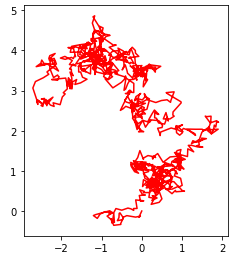
\includegraphics[width = 0.25\textwidth, clip = false]{Figs/SingleBPplot.PNG}
	\end{figure}
	
	We're working with a stochastic system here, so obviously your plot won't look exactly the same as this, however it should be similar. If not, you may wish to look back over your \texttt{moveBrownianParticle} function.
	
	\subsection{Defining the RMSD function}
	
	The Root Mean Squared Displacement $r$ is typically used to determine the macroscopic diffusion coefficient $D$. In 2D, it is defined as
	
	\begin{equation}
		r(t) = \langle(x(t_0 + t)-x(t_0))^2 + (y(t_0 + t)-y(t_0))^2\rangle,
	\end{equation}
	
	where $\langle \cdot \rangle$ indicates the average over all particles and all reference times $t_0$ and $t$ is the lag time. This function is already coded up for you in \texttt{BrownianMotionFunctions.py}.
	
	\subsection{Is $r \propto \sqrt{t}$?}
	
	We can now run a number of independent simulations and calculate the RMSD of the resulting trajectories. How can we check if the prediction $r \propto \sqrt{t}$ holds? One way is to take logs of both sides:
	
	$$\log(r) \propto \log(t^{\frac{1}{2}})$$
	
	$$\implies \log(r) \propto \frac{1}{2}\log(t)$$
	
	\noindent
	In other words, if we plot $\log(r)$ against $\log(t)$, the resulting line should have a slope of 1/2. Let's check this:
	
	\bigskip
	
	\textbf{Exercise 2:} Perform 10 independent simulations by inserting code at the indicated position in \texttt{BrownianMotionSimulationRMSDcheck.py} and running the script. If you have implemented your simulations correctly, you should see a blue line (containing the data from your simulations) and a black reference line with slope $\frac{1}{2}$. Please include this in your write up. Is our theoretical prediction supported by these simulations?
	
	\bigskip
	
	\section{Investigating the diffusion coefficient $D$}
	
	According to the Stokes-Einstein equation, the diffusion constant $D$ and absolute temperature $T$ of a diffusive system are related by:
	
	\begin{equation}
		D = \frac{kT}{6\pi\mu a},
	\end{equation}
	
	\noindent
	where $k$ is Boltzmann's constant, $\mu$ is the dynamic viscosity of the liquid and $a$ is the particle radius. In this exercise, we will vary the temperature of our particles while keeping the particle size and fluid viscosity constant. For our purposes, we can therefore rewrite this prediction as:
	
	\begin{equation}
		D \propto T.
	\end{equation}
	
	\noindent
	Note that the equations we used to define our \texttt{moveBrownianParticle} function were dependent on $T$. We are therefore asking whether we understand the connection between what we define at the microscopic level ($T$) and the behaviours that emerge at the macroscopic level ($D$).
	
	Let us recall from the lectures that, in 2D,
	
	\begin{equation}
		r^2 = 4Dt.
	\end{equation}
	
	\bigskip
	
	\textbf{Exercise 3:} Plot $r^2$ versus $t$ and verify that the relationship between them is linear. What gradient do you predict this line will have?
	
	\bigskip
	
	We can therefore estimate $D$ as 
	
	\begin{equation}
		D = \frac{r^2}{4t}.
		\label{eq:Dest}
	\end{equation}
	
	\bigskip
	
	\textbf{Exercise 4:} Using equation \ref{eq:Dest}, estimate the value of $D$ for your simulations. To obtain a single value, you can take the average across all values of $t$. 
	
	In the lectures, you saw that $D$ could be also be calculated as $\frac{\delta^2}{2\tau}$, where $\delta$ is the size of a single step and $\tau$ is the time it takes for the direction of motion to be randomised. Estimate $D$ using this equation. How does it compare to the value you just calculated based on the simulations? (\textit{Hint:} The \textit{average} step size is $\approx 1.12 \sqrt{T} \Delta t$, as the average magnitude of a two component vector where both elements are drawn from a standard normal distribution $\approx 1.12$. You can use this as your value of $\delta$.) 
	
	\bigskip
	
	\subsection{Optional exercise 5: Investigating the relationship between $T$ and $D$}
	
	If you have time after completing the above exercises and fancy more of a challenge, please work on the problem below. (This section is just for fun, not for credit)
	
	In the previous exercises, you have seen how to run simulations of particles undergoing Brownian motion (Exercise 1), how to calculate the RMSD of these particles (Exercise 2), and how to calculate $D$ from the RMSD (Exercise 4). With these tools, you should now be able to investigate the relationship between the diffusion coefficient $D$ and the temperature $T$. 
	
	Plot the values of $D$ derived from simulations with different values of $T$. What do you predict the relationship between these two quantities will be? Why do you think it might be useful to experimentally measure this relationship?
	
	\textit{Hint:} here is some pseudocode to help you organise your code:
	
	\begin{enumerate}
		\item Create a list of temperature values that you will test over
		\item Preallocate some storage for the value of $D$ associated with each temperature
		\item Loop over temperatures
		\begin{enumerate}
			\item Preallocate some storage for the simulated particle positions at this temperature
			\item Loop over particles
			\begin{enumerate}
				\item Initialise a new particle at the origin (0,0)
				\item Simulate particle movement (i.e. loop over time) and store particle positions at each timepoint
			\end{enumerate}
			\item Calculate $r$ for this set of simulations
			\item Caculate the mean value of $\frac{r^2}{4\tau}$ for this set of simulations and store this as $D$
		\end{enumerate}
		\item Plot $T$ vs. $D$
	\end{enumerate}
	
	Note that steps (a)-(d) are similar to what we did to complete exercise 4.	
	
\end{document}
